\documentclass[11pt,a4paper,openright]{report}

\usepackage{float}
\usepackage{booktabs}
\usepackage[margin=0.9in]{geometry}
\usepackage[moderate]{savetrees}
\usepackage{graphicx}
\usepackage{enumitem}
\usepackage{titlesec}
\usepackage[svgnames]{xcolor}
\usepackage[colorlinks=true, linkcolor=blue, urlcolor=blue, citecolor=red]{hyperref}
\usepackage{caption}
\usepackage{subcaption}
\usepackage{amssymb}
\usepackage{pifont}
\usepackage{array}

% Referencing macros
\newcommand{\Eqref}[1]{Equation~\eqref{#1}}
\newcommand{\Tabref}[1]{Table~\ref{#1}}
\newcommand{\Figref}[1]{Figure~\ref{#1}}
\newcommand{\Appref}[1]{Appendix~\ref{#1}}
\newcommand{\putiitblogo}{
\includegraphics[width=10em]{iitb-black}}
\newcommand{\cmark}{\ding{51}}%
\newcommand{\xmark}{\ding{55}}%
\newcolumntype{P}[1]{>{\centering\arraybackslash}p{#1}}

\newcommand{\myparagraph}[1]{\paragraph{#1}\mbox{}\newline\newline	}

% Table of contents display
\setcounter{tocdepth}{3}
\setcounter{secnumdepth}{3}

% Formatting
\titleformat{\chapter}{\normalfont\huge\bf}{\thechapter.}{20pt}{\huge\bf}
\linespread{1.05}
\setlength{\parindent}{2em}
\setlength{\parskip}{0.3em}
\setitemize[0]{leftmargin=2em,itemindent=0.5em}
\setlist[enumerate]{itemsep=0mm}
\setlist[itemize]{itemsep=0mm}

\begin{document}

  % Coverpage
  \begin{titlepage}    
    \begin{center}
   
      \Large \textbf{Adapative memory management framework \\for derivative clouds}  \\
      \vspace{5em}
      
      \large \textbf{Master's Thesis Report} \\
      \vspace{5em}
      
      \normalsize A thesis \\submitted in partial fulfillment of the \\requirements for the degree of \\
      \vspace{1em}      
      \large \textbf{Master of Technology} \\
      \vspace{5em}
      
      \normalsize by \\
      \vspace{1em}      
      \large \textbf{Prashanth} \\ 
      \vspace{0.5em}
      \normalsize Roll No: 153050095 \\
      
      \vspace{5em}
      \normalsize under the guidance of \\
      \vspace{0.5em}      
      \large \textbf{Prof. Purushottam Kulkarni} \\
      \vspace{5em}
      
      \putiitblogo \\
      \Large 
      Department of Computer Science and Engineering \\
      Indian Institute of Technology, Bombay \\
      Mumbai
      
    \end{center}
  \end{titlepage} 
  
  \begin{center}
    \huge \textbf{Abstract}
  \end{center}
  \vspace*{3em}
  \normalsize 
    Cloud computing has emerged as one of the hot topics in the computing community today. Most servers these days are either 
already running on cloud, or are in the virtue of shifting base to cloud. Cloud providers traditionally multiplex a set of compute 
resources, to group of isolated clients using hardware level virtualization techniques that make use of Virtual Machines (VM) to deploy 
isolated Virtual Environments (VE). 

    Although VMs provide a very effective methodology in provisioning compute over the cloud, they incur heavy overheads there by degrading 
efficiency while provisioning. Lately, there has been a new direction in the flow of research in virtualization, i.e OS-level virtualization 
in which compute resources in a system are virtualized at an OS-level to provision light weight isolated VEs called Containers. Containers 
provide similar features to that as VMs but incur much lesser overheads \cite{felter2015updated} \cite{morabito2015hypervisors} . A recent 
work \cite{sharma2015spotcheck} has also tried to take it a step ahead, by provisioning compute resources to clients using an nested 
approach in which repackages and resells resources purchased from native Infrastructure-as-a-service (IaaS) cloud provider. This approach is 
coined as derivative cloud.

    In this work, we have made an initial attempt to understand memory management between containers. We started off with purposing 
hypotheses based on theoretical evidences. We performed analysis to verify the correctness of our purposed hypotheses and understand parts 
of memory management for which hypotheses couldn't be drawn. We then tried to extrapolate its implications on real world applications 
running inside a derivative cloud environment running VMs on the host machine and containers in the guest machine. These implications 
strongly suggested that existing memory management techniques may impact higher provisioned containers negatively. We conclude by purposing 
the requirements of a new desired policy that provides this notion of a differentiated reclamation to enforce deterministic allocation when 
the system is under memory pressure. The end goal of our work is to provide an adaptive deterministic resource provisioning framework for 
container based services. 




    
  \pagenumbering{roman}
  \tableofcontents
  \listoftables
  \listoffigures
  \cleardoublepage
  \setcounter{page}{1}
  \pagenumbering{arabic}
  \setlength{\parskip}{1em}
  
  \chapter{Introduction}
  
  The present era has observed extreme levels of inflation in the number of compute systems being used to automate day to day tasks. 
Historically this process of automation was typically carried over a system existing locally. However, the past couple of 
decades has witnessed an hostile take over by \textit{The Internet}, which has been helpful in connecting systems over the 
globe. Overtime, several businesses have started offering computational resources as a service, over the Internet. This has lead to 
the establishment of a new paradigm of computation known as \textit{Cloud Computing} or simply the Cloud and such businesses are called 
cloud service providers. 

  The objective of a customer is to run his application on the cloud without affecting the performance of his application. On the 
other hand, the objective of a cloud provider is to minimize running costs when serving multiple such customers with promised guarantees to 
make their business profitable. This leads to conflicting goals between the provider and the customer. How this is handled would 
be discussed in the next section. 

Providers today offer various kinds of cloud services like Software as a service (SaaS), Platform as a service (PaaS) and Infrastructure as 
a service (IaaS). SaaS provides software applications being run on a cloud server. PaaS supports the complete life cycle of building and 
delivering applications. IaaS provides basic compute resources as a service, and is considered as the most primitive form of providing 
cloud services. Most of our discussions would be centered with having IaaS in mind although the findings could be extrapolated to either of 
the services types mentioned here. A recent study \cite{forbes} suggests that 75\% of the corporates are migrating to using the cloud to 
run their businesses, and also that by 2020 all corporates would be using cloud services similar to how the Internet is used today.   

  The emergence of cloud computing paradigm has opened gates to a new direction for flow of Systems research. Traditional systems were 
developed to only serve a single or a group of trusted users. Now with multiple untrusted users existing on a single system has 
lead to changing the focus of improving efficiency, manageability, service guarantees over a group of isolated customers, who have to be
protected from being affected by other customers running on the same system. One of the common ways to achieve this is using 
\textit{Virtualization}. Virtualization seems to be the most effective and secure way of achieving this. Virtualization has several 
techniques used but the two techniques we would be focusing are Hardware level virtualization using \textit{Virtual Machines} (VM) and 
Operating System level virtualization using \textit{Containers}.

  \section{Deterministic resource provisioning for cloud services}
  
    Most commonly provisioned resources are compute, storage, network and memory. Most cloud services make use of hardware level 
virtualization techniques that use Virtual Machines to provision compute resources as per client requirements. Such use of virtual machines 
has been done for over a decade now and have gotten relatively stable and secure. Earlier resources were provisioned by cloud providers 
were static, however static provisioning leaves less room for server consolidation hence providers are moving to a more elastic on-demand 
model where resources provisioned are over-committed to a group of customer and servers are provisioned as per actual resource needs. A 
popular example for the same is Amazon's EC2 \cite{amazonec2} that offers elastic web services which expand or compress as per actual 
needs. Elastic provisioning of resources in a virtualized environment is more tricky task and leads to a lot of non-determinism. 

    There are several advanced resource provisioning techniques \cite{dornemann2009demand} \cite{shen2011cloudscale} 
\cite{moreno2009elastic} \cite{calheiros2012aneka} etc. using virtual machines that make use of horizontal/vertical provisioning techniques 
to satisfy client QOS (quality of service) requirements at the same time perform server consolidations to reduce operating costs. However, 
hardware level virtualization layer induces overheads that are caused by dual control loop while scheduling resources, complete hardware 
stack emulation for each VM, resources used by the hypervisor (entity that manages VMs) etc. These overheads lead to bad cost-benefit ratios 
which adversely affects customers by overpricing services offer by cloud provider.
  
    A recent trend in virtualization has been towards OS-virtualization that makes use of lightweight containers to provision resources. 
Several researches \cite{felter2015updated} \cite{morabito2015hypervisors} \cite{agarwal2015containing} \cite{beserra2015performance} 
\cite{rathore2013kvm} have shown that containers provide provide near about the same features (with a few limitations) as that of virtual 
machines but with much lesser overheads. Static provisioning using containers can be done easily today, however deterministic provisioning 
of containers is still to be explored in depth specially in situations of overcommitment. Containers are relatively a young technology that 
needs further refinement to be used in deployment. Several enterprises are hesitant to move towards containers due to the existing security 
issues. More about containers shall be provided in the coming chapters.

    \begin{figure}
      \centering
      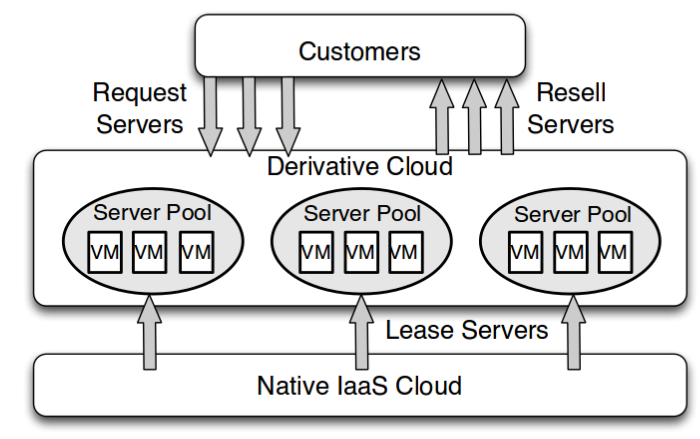
\includegraphics[width=0.7\textwidth]{images/intro/derivative_cloud.png}
      \caption{Depiction of a derivative IaaS cloud platform, Source:\cite{sharma2015spotcheck}}
      \label{img_derivative_cloud}
    \end{figure}

    This idea of deterministic provisioning can be expanded to a \textit{derivative cloud} environment as purposed by P.Sharma in his 
recent work \cite{sharma2015spotcheck} which repackages and resells resources purchased from native IaaS platforms. A derivative cloud can 
offer resources to customers with different pricing models and availability guarantees not provided by native platforms using a mix of 
resources purchased under different contract. Derivative cloud providers rent resources from native cloud providers to resell services to 
customers as shown in Fig:\ref{img_derivative_cloud}.

    Although containers support has been provided in most major operating systems today, it is most popular and widely used in operating 
systems running on a Linux kernel. Our entire work would focus on elastic provisioning of containers in a native Linux environment and 
extend its implications to the derivative setup. However at this stage, we focus on deterministic provisioning of memory and disk-caching 
as a resource in this thesis.

  \section{Memory management in clouds}
  
    Memory as a resource has gained popularity recently with emergence of more memory intensive applications in various fields of 
computing like data analytics, caching that have a very strong correlation with application performance that is dependent on the memory 
available in the system. Most memory sensitive applications constantly use any unused memory available in the system to benefit them. A 
simple example is an Key-value used to cache frequent key's accessed by a web application. 

    Currently available provisioning knobs in the Linux container framework are quite effective while provisioning for applications when 
the host system isn't under any memory pressure and overcommitment (When resources promised on a system is more than resources available). 
However overcommitment is a fundamental requirement to provision cloud servers to maximize provider running costs as discussed earlier. In a 
native Linux system, memory pressure might be generated due to the following 

      \begin{enumerate}
	\item Additional memory required by processes of other containers
	\item More memory required by processes/services running on host Linux OS
	\item Memory pressure generated by kernel threads/processes
      \end{enumerate}
      
      Let's see how memory overcommitment and pressure can disrupt desired functionality of the existing container framework provided by 
Linux containers.

    \subsection{Issues in native container environment}	
    
    Consider two containers provisioned for running Mongo-DB containers from 2 different customers on a same host machines. Now that 
average memory used by the 2 containers are in the ratio of 1:2 and the customers for the 2 containers are also paying for their services in 
the same ratio. Let's call container with 1x workload usage as Mongo-Low and that of with 2x usage as Mongo-High. Now assume the customers 
have been provisioned using existing memory knobs with the same ratio as shown in Tab:\ref{table_initial}. For the sake of simplicity assume 
that all the containers over-provisioned for all other resources and aren't throttled by any other resource. Low and High can be thought of 
relative priorities of each of the containers.
	
	\vspace*{1em}	
	\begin{table}[!h]
	  \begin{center}
	    \begin{tabular}{ l | p{3cm} | p{2.2cm} | p{2.2cm} | p{2.2cm} }	      	    
		  & Average Memory Usage & Cost Paid for Service & Memory Provisioned & Desired Throughput \\ 
	      \hline
	      \hline
	      Mongo-Low  & 1x & 1x & 1x & 1x \\  
	      \hline
	      Mongo-High & 2x & 2x & 2x & 1x \\
		
	    \end{tabular}
	  \caption{Memory Provisioned for the Containers using existing memory provisioning knobs}
	  \label{table_initial}
	  \end{center}	  
	\end{table}
	\vspace*{1em}
	
	\pagebreak
	
	\begin{figure*}[t!]
	  \centering
	  \begin{subfigure}[t]{0.48\textwidth}
	    \centering
	    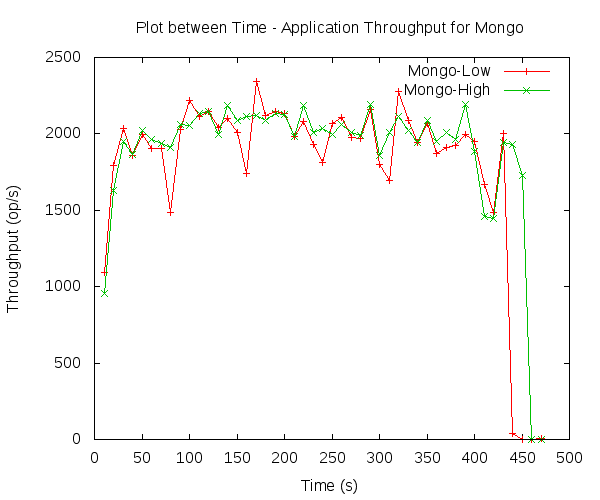
\includegraphics[width=1\textwidth]{images/intro/native.png}
	    \caption{Running applications without containers}
	    \label{plot_intro_native}
	  \end{subfigure}
	  ~ 
	  \begin{subfigure}[t]{0.48\textwidth}
	    \centering
	    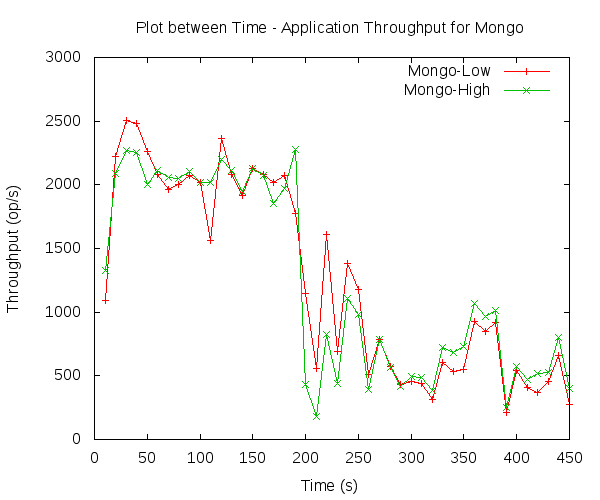
\includegraphics[width=1\textwidth]{images/intro/observed.png}
	    \caption{Observed after provisioning containers using existing knobs}
	    \label{plot_intro_observed}
	  \end{subfigure}
	  ~ 
	  \begin{subfigure}[t]{0.48\textwidth}
	    \centering
	    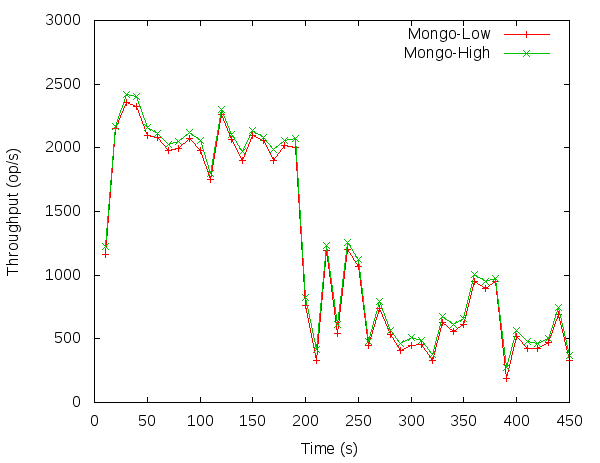
\includegraphics[width=1\textwidth]{images/intro/desired.png}
	    \caption{Desired after provisioning containers using knobs}
	    \label{plot_intro_desired}
	  \end{subfigure}
	  \caption{Application throughputs for problem establishment}
	\end{figure*}
	
	Consider 3 cases as described below. In cases 2 and 3, containers are allowed to run normally for about 100s and there after 
which free memory in the system gradually reduces by generating of memory pressure by an external entity. 
	
	\begin{itemize}
	  \setlist{nosep,after=\vspace{\baselineskip}}
	  \item Case-1: Running applications natively in a system with 1:2 memory assignments and no pressure 
	  \item Case-2: Observed throughputs after provisioning with existing knobs under pressure
	  \item Case-3: Desired throughputs under pressure
	\end{itemize}
	
	Fig:\ref{plot_intro_native} shows the simple case where both the containers achieve desired throughputs when running on a system 
with no container specific provisioning. The containers start execution with no memory pressure and hence must be able to each equal 
throughputs initially in all 3 cases although. Case-2 still shows lower levels of application performance for higher provisioned 
containers even when the system is under no pressure. In observed throughputs under pressure Fig:\ref{plot_intro_observed}, we 
observe that throughputs of Mongo-High (Container with higher priority) is negatively affected at some point or the other, when in reality 
its throughput had to be better if not same as shown in Fig:\ref{plot_intro_desired} considering its higher resource allocations. 
	
	\pagebreak

	\begin{table}
	  \begin{center}
	    \begin{tabular}{ l | c | c | c }	      	    
		  & No Pressure & Observed & Desired \\ 
	      \hline
	      \hline
	      Mongo-Low  & 1825 & 1268 & 1255$-$ \\  
	      \hline
	      Mongo-High & 1972 & 1242 & 1255$+$ \\
		
	    \end{tabular}
	  \caption{Average throughput in each case (op/s)}
	  \label{table_intro_th}
	  \end{center}	  
	\end{table}
	
	Table:\ref{table_intro_th} shows how average throughputs vary in each case. It can be seen that the average throughput in case-2 
which is the provisioning of containers using existing knobs may negatively impact containers with higher allocations. By looking at the 
example here, we can conclude by saying that 
	
	\begin{enumerate}
	  \item Native memory allocations work well with containers where there doesn't exist any memory overcommitment and pressure
	  \item However when the two occur, memory reclamation may adversely affects containers which are better provisioned (since they 
were promised higher QOS) than those which aren't.
	\end{enumerate}
    
    \subsection{Amplification of issues in derivative cloud environment}
      
      Considering the above described setup to derivative cloud where the native cloud provider is using VMs to provision customer demands. 
This VM acquired from the native cloud provider is again repacked and resold by the derivative cloud provider to specific customers. In 
this case, this situation further complicated due to two reasons,
      
      In the native case, memory overcommitment was a required condition for the previously described situation to arise. Consider the case 
where all containers were assigned memory considering the available system memory in such a way that there is no overcommitment, however 
now the native cloud provider (host system) could reduce the memory available to the system using different memory reclamation policies at 
the host.
       
       \begin{enumerate}
	  \item Memory overcommitment is not a required condition
	  \item Memory pressure maybe introduced by three factors described earlier or an additional factor like an external host system 
driver (eg: Balloon Driver)
       \end{enumerate} 

      The reclamation could be trigger by a host driver like the \textit{Balloon Driver} that is widely used by the \textit{Hypervisor} 
(Entity that manages VMs) by cloud providers. This leads to further discrepancies in the memory management at the container level. 
  
  \section{Caching in the cloud}
    Caching of data has played a crucial role in provisioning for applications on the cloud. Caching provides a faster
    mechanism to access frequently accessed data. There are several web services these days that make use of CDNs (content 
    distribution networks) to cache their frequently accessed to minimize response time by spreading these CDNs servers across
    the globe. This is one form of commonly used caching frameworks. Another form of caching occurs at the application level
    where frequently accessed key-value pairs are stored in a key-value store like Redis \cite{redis}, Memcached \cite{memcached}.
    However our work deals with cloud frameworks where the cloud provider caches client data to improve client performance.
    Let's begin with how caching occurs in a traditional cloud setup.
    
   \subsection{Drawbacks of caching in traditional (VM) cloud setup}
      
     \begin{figure}
      \centering
      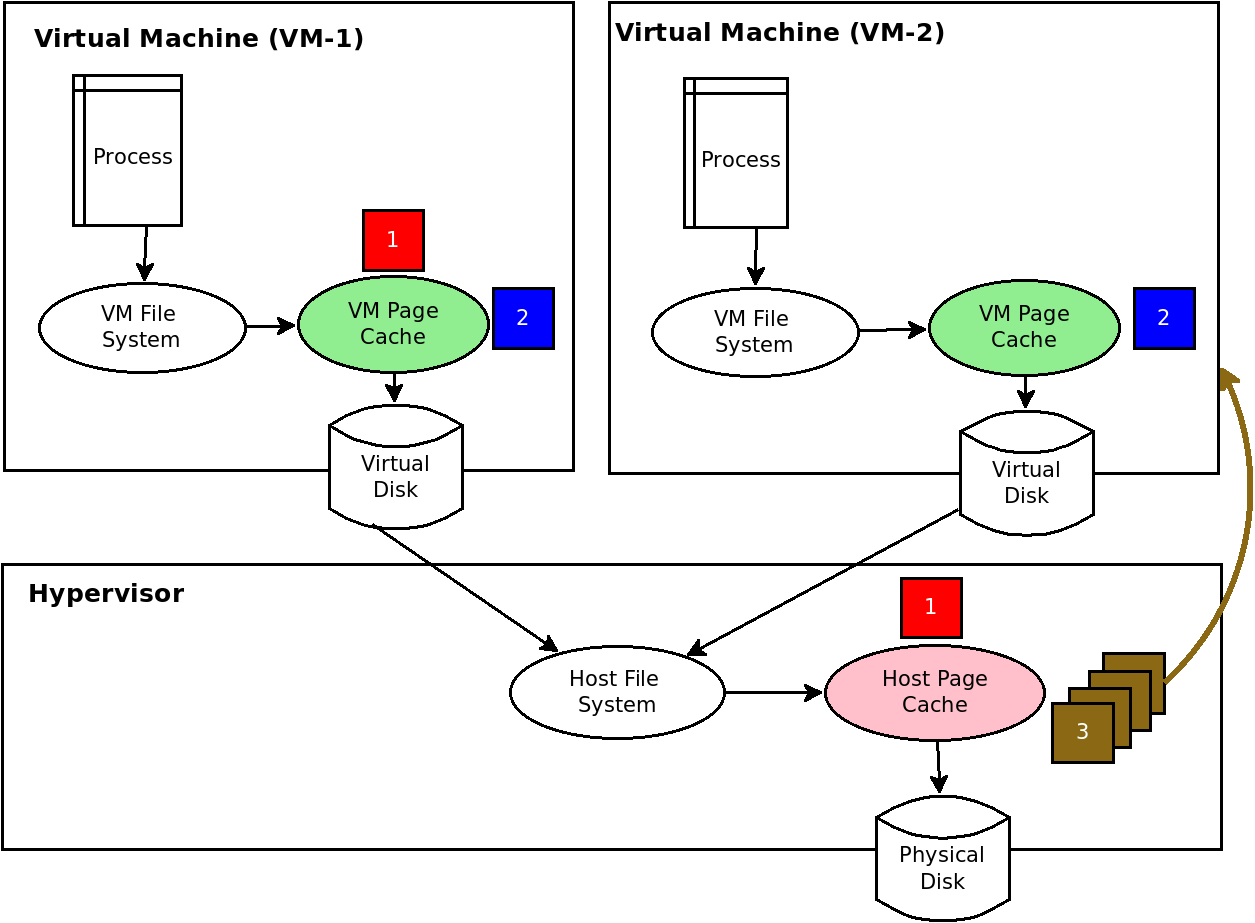
\includegraphics[width=0.8\textwidth]{images/intro/issues_in_hypervisor.png}
      \caption{Drawbacks of caching in traditional VM cloud setup}
      \label{img:drawbacks_traditional}
    \end{figure}
    
    Fig~\ref{img:drawbacks_traditional} depicts a traditional host page caching at occurs in a virtualized setup. There are
    two-levels of caching occurring here, one at the guest and the other at the host level. 
    Both these caches are controlled by their respective operating systems and are unaware of one another.
    This leads to improved performance but will also lead to wastage of resource. 
    The drawbacks of such a setup are (as illustrated in Fig~\ref{img:drawbacks_traditional} listed below,
    
      \begin{enumerate}
	\item A copy of the same page is present at the hypervisor page cache and the VM page cache.
	\item A copy of the same page maybe present across VMs.
	\item The host page cache could be flooded with page caches from a single or a set of VMs.
      \end{enumerate}
      
   \subsection{Hypervisor managed caching}
    
    To overcome above drawbacks, several works\cite{mishra2014comparative, koller2015centaur} have proposed the use of
    a more controlled caching framework called the \textit{Hypervisor managed caches} as depicted in Fig~\ref{img:hc}.  
    Hypervisor managed caches are caching frameworks whose control lies in the hands of the native cloud provider. 
    The native cloud provider cloud provision these caches to satisfy an application level objective which could be 
    exposed as a service to their clients or also to configured based on a global provider level policy to maximize 
    throughput.
    
      \begin{figure}
	\centering
	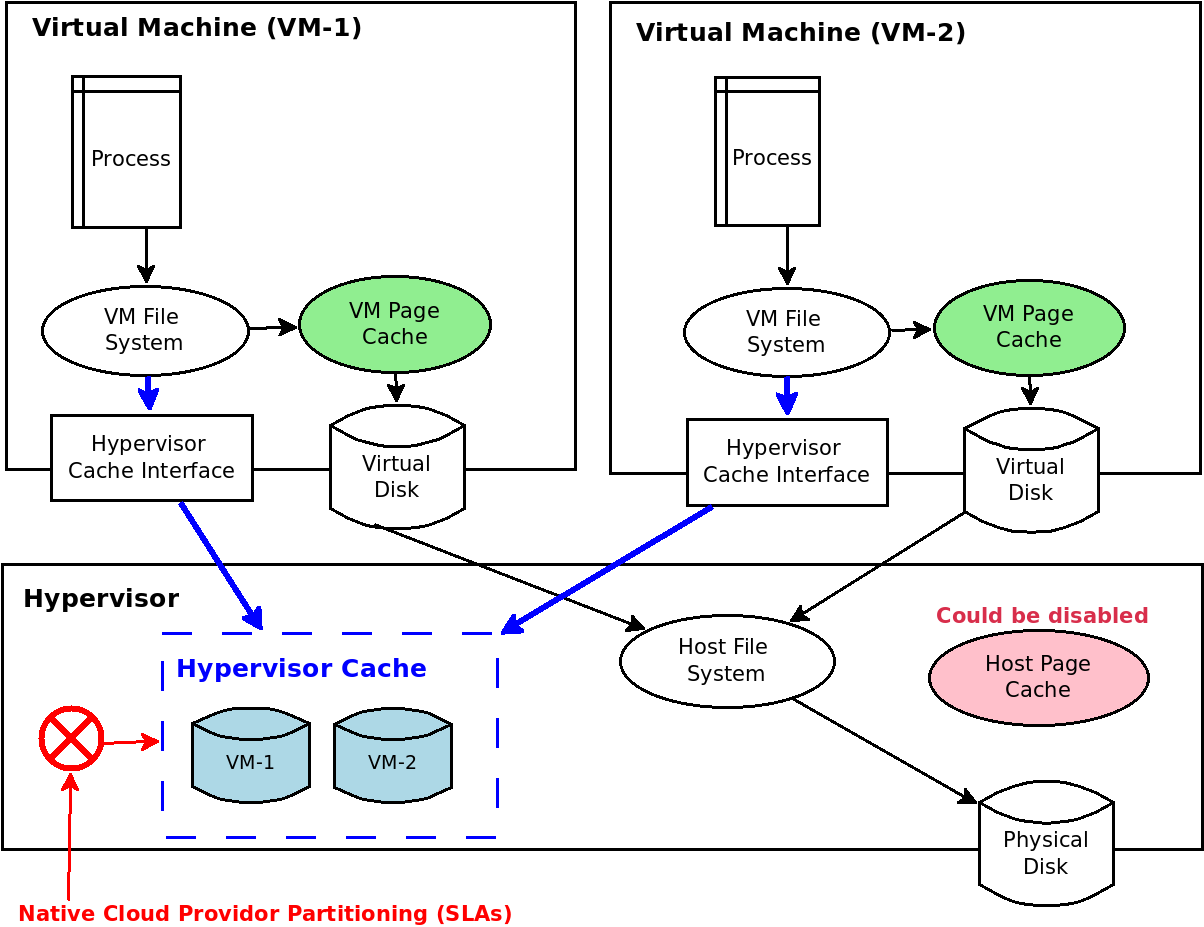
\includegraphics[width=0.8\textwidth]{images/intro/hc.png}
	\caption{Hypervisor managed cache}
	\label{img:hc}
      \end{figure}    
    
    Hypervisor managed caches eliminates the drawbacks previously discussed by providing an exclusive cache there by 
    removing any redundant pages. The cache size can be configured there by eliminating flooding of page cache by a single
    VM. Typically host-side page cache is turned off when hypervisor managed cache is enabled.
    
    \subsection{Issues of caching frameworks in derivative clouds}
      Hypervisor managed caches have shown significant improvements in performance improvements in a native cloud environment, 
      but however when it comes to derivative clouds the existing frameworks aren't able to differentiate the nested levels
      of virtualization entities. Existing cache partitioning frameworks\cite{koller2015centaur, stefanovici2015software}
      that partition caches for each VM assumed a single application running and hence successfully partitions the same, 
      however with multiple applications running in an derivative setup, cache partition to achieve application objectives 
      (SLAs) becomes challenging as shown by \dd{}\cite{doubledecker}. \dd{} was the preliminary work done based on which 
      this work is built upon, however even with \dd{} like other caching frameworks there exist drawbacks as discussed 
      below.
      
      \subsubsection{Lack of framework support in derivative clouds}
	Caching frameworks existing lack support for derivative clouds. They lack the engineering components required to 
	exposed container as an individual provisioning entity. \dd{} addressed this by exposing cache provisioning to a
	derivative cloud provider. A similar approach could be used for other partitioning frameworks as well.
      
      \subsubsection{Dual layers of isolated control}
	With a caching framework like mentioned above incorporated into a derivative cloud setup makes it have two isolated
	control centers - one at the native cloud provider level (hypervisor) and the other at the derivative 
	cloud provider (VM) level. The native cloud provider is only responsible for partitioning the cache, where as the 
	derivative cloud provider is responsible for distributing the VM memory among the container. Such isolation makes
	it difficult for a derivative cloud provider to get a holistic view while provisioning for application objectives. 
	
      \subsubsection{Application cache sensitivity is unaccounted}
	With two levels of memory provisioning - In-VM and hypervisor cache makes it challenging to provision applications 
	has some applications have specific needs of In-VM requirements whereas the others are more flexible about it. 
	Caching frameworks fail to address this issue.
    
  \section{Problem description}  
    Keeping the above drawbacks in mind, the following are the outline of the problem description for our work. 
  
   \subsection{Memory management for containers}
      In the initial phase of our work we wish to 
      \begin{enumerate}
	\item Understand the existing memory management policies used by Linux to manage containers.
	\item Identify issues with existing policies and purpose new policies to be supported for.
	\item Do the same for both native and derivative cloud environments. 
	\item Design a solution to support purposed policies and empirically evaluate its correctness.
      \end{enumerate}

   \subsection{Holistic cache and memory management for containers}
      In this phase of our work we wish to
      \begin{enumerate}
	\item Understand existing cache partitioning frameworks.
	\item Identify issues with the existing frameworks.
	\item Come up with solution to fix identified issues and empirically evaluate its correctness.
      \end{enumerate}

  \section{Contributions}
    The following are the contributions of our work.  
      \begin{enumerate}
	\item Built a differentiated memory management controller for containers. This work has been 
	accepted in \textit{IEEE ICDCS '17} for the poster track.
	\item Designed and implemented an decentralized memory (and cache) management framework for containers. This work 
	is in submission at \textit{ACM Middleware '17}.
      \end{enumerate}

    
  \chapter{Background}

  
  \section{Memory management between processes in Linux}
  
    Memory is allocated/deallocated in terms of pages in any operating system. Memory management in Linux is done using techniques like 
virtual memory, demand paging, swapping caching etc. They separate between the memory needed by a process and the memory physically 
allocated on the RAM. The OS creates a large virtual address space for each process. In this section we focus on how memory is managed 
between processes or a group of processes. We mainly focus on how memory is assigned and reclaimed between them.  
  
    \subsection{Memory pages used by a process}
      Memory used by processes are divided into 2 types of pages	
      \begin{enumerate}	
	\item Anonymous Pages: Pages those which are not associated with any files on disk. They are process memory pages.
	\item Page cache pages: Are an in-memory representation of a part files on the disks.	
	\item Mapped pages: File page with VA mappings
      \end{enumerate}
  
    \subsection{Memory allocation}
      When the process needs memory to be allocated, Linux decides the how this memory is going to be allocated physically on the RAM. The 
process/ application does not see in physical RAM addresses. It only sees virtual addresses from the virtual space assigned to each process.
The OS uses a page file located on the disk to assist with memory requests in addition to the RAM. Less RAM means more pressure on the Page 
file. When the OS tries to find a piece of memory that's not in the RAM, it will try to find in the page file, and in this case they call it 
a page miss. The actual physical memory allocated (RSS) to a process depends on how much free memory is available in the system. On free 
memory becoming freshly available in the system, the OS tries to equally distribute the available memory to all processes that are 
demanding for more memory.

    \subsection{Memory reclamation without container support}
      Two lists 
      
  \section{Containers}
    \subsection{Control groups (Cgroups)}
      \subsubsection{Memory Cgroup}
	\paragraph{Memory reclamation with Cgroups}
      
  
  \section{Caching}
  
   \subsection{Hypervisor managed caching}
      \subsubsection{T-MEM cache}
    
   \subsection{Multilevel caches}
    
   \subsection{Application specific cache partitoning}
      \subsubsection{MRC construction}
      
   \subsection{Double decker: Second chance cache for derivataive clouds}
  
      

       
  %
\chapter{Related work}

  There have been several attempts to provide efficient memory management for virtual machines. The most prominent used approach is of 
that Ballooning \cite{waldspurger2002memory}. Ballooning is an mechanism that reclaims pages considered least valuable by the guest OS 
running inside the virtual machine. This allows the VM to decide which memory pages to release instead of the host trying to determine this.
Gerḿan Molt́o \cite{molto2013elastic} expands the idea of Ballooning to provide a system to monitor the VM memory and apply vertical 
elasticity rules in order to dynamically change its memory size by using the memory ballooning technique provided the KVM hypervisor. 
Overdriver \cite{williams2011overdriver} on the other hand presents a system that handles all durations of memory overload. It adapts its 
mitigation strategy to balance the trade offs between migration and cooperative swap to handle memory overcommitments. Ex-Tmem 
\cite{venkatesan2014ex} stores clean pages in a two-level buffering hierarchy with locality-aware data placement and replacement. It 
enables memory-to-memory swapping by using non-volatile memory and eliminates expensive I/O caused by swapping.
  
  Looking at researches that have looked at resource provisioning, CloudScale \cite{shen2011cloudscale} can resolve scaling conflicts 
between applications using migration, and integrates dynamic CPU voltage/frequency scaling to achieve energy savings with minimal effect on 
application SLOs. Tim Dornemanna\cite{dornemann2009demand} proposed a solution that automatically schedules workflow steps to underutilized 
hosts and provides new hosts using cloud computing infrastructures in peak-load. The system was based on BPEL to support on-demand resource 
provisioning. Aneka \cite{calheiros2012aneka}, is a platform for developing scalable applications on the Cloud, that supports provisioning 
resources from different sources and supporting different application models. It support the integration between Desktop Grids and Clouds. 
Elastic Application Container (EAC) \cite{he2012elastic} is a virtual resource unit for delivering better resource efficiency and more 
scalable cloud applications. 

  A derivative cloud is a nested setup, virtual machines nested in virtual machines\cite{williams2012xen} or containers deployed in virtual machine 
  \cite{sharma2015spotcheck, gcp}, the latter being the focus of this work.  

  There has been extensive work carried out in hypervisor caching\cite{lu2007virtual, magenheimer2009transcendent, mishra2014comparative, schopp2006resizing}.
  On top of this there has been work carried out to partition hypervisor caches based on application SLAs \cite{schopp2006resizing, koller2015centaur}.

  Although there are several existing works in elastic resource provisioning (including memory) for virtual machines as listed above. There 
  has been no attempt to provide an deterministic memory management policy for containers. To our knowledge this is our first attempt to do 
  so.
  
  Applicability of hypervisor caching in a derivative cloud setup is hindered due to inability of existing frameworks to support this sort of
  provisioning, and also we would like to look at the overall picture of memory management at all levels of the hierarchy along with the cache
  partitioning to satisfy application SLA. 

%   \subsection{Hypervisor managed caching}
%       \subsubsection{T-MEM cache}
%     
%    \subsection{Multilevel caches}
%     
%    \subsection{Application specific cache partitoning}
%       \subsubsection{MRC construction}
%       
%    
  
\chapter{Differentiated memory management controller for containers}

  Overview here
  
  \section{Drawbacks of existing memory management for containers}
  
    \subsection{Issues in native environment}
    
      \subsubsection{Reclamation above soft limits}
      
      \subsubsection{Reclamation below soft limits}
   
    \subsection{Amplification of issue in derivative clouds}
  
  
   
  \section{Requirements for a new memory management controller}
      
    
  
  \section{Proposed memory management controller}
    
      \subsection{Controller architecture}
    
      \subsection{Policies supported by the controller}
	
  
  
  \section{Modifications made to Linux memory Cgroup}
  
    \subsection{Per container configurable weights}
    
    \subsection{Deterministic reclamation}
    
    \subsection{Flexible reclamation size}
    
  
  
  \section{Empirical evaluation of our controller}
  
    \subsection{Effectiveness of our controller}
    
    \subsection{Differential QOS containers}
    
    \subsection{Impact of reclamation chunk size}
  \chapter{Double decker: A memory management framework for derivative clouds}



  \section{Application cache sensitivity}
  
    \subsection{Provisioning of caches at different levels based on application sensitivity}
    
    \subsection{Inability of cache partitioning framework to support anonymous memory applications}
    
    

  \section{Rethink of existing design}
  
    \subsection{Decentralized memory management framework}
	      
      \subsubsection{Native provider cache partitioning framework}

      \subsubsection{Derivative provider memory management framework}	

    \subsection{Hybrid cache}
      
      \subsubsection{Multilevel configurable caches}
      
      \subsubsection{Movement of cache objects}
      
	
  
  \section{Implementation details}
      
    \subsection{Existing implementation status}
    
    \subsection{Hybrid cache}
    
      \subsubsection{Pools to accommodate both memory and SSD objects}
      
      \subsubsection{Asynchronous kernel threads for movement of objects}
      
      \subsubsection{Multilevel stats}
  
  \newpage
  
  \section{Correctness of implementation}
  
    \subsection{Experimental setup}
	
      The following section describes the experimental setup used to verify the correctness of our implementation. 
	
      \myparagraph{Experimental configurations}	
	The set of configurations used for an analysis of memory management framework for a derivative environment must be relevant, and easy to apply. The following configurations
fit this criteria, and have been used for the evaluation.

	  \begin{itemize}
	   \item \textbf{Memory Requirement:} Memory requirement of each container, the estimated total memory used by a container.
	   
	   \item \textbf{Container memory limit:} Size of memory allocated to a container at the Cgroup level (soft and hard limits). 
	   \item \textbf{Memory cache limit:} Size of memory (L1) cache assigned to a container. 
	   \item \textbf{SSD cache limit:} Size of SSD (L2) cache assigned to a container.
	   
	   \item \textbf{Workload:} Workload application that is running inside each of the container. 
	   \item \textbf{Number of containers:} Number of containers that are currently executing in the system.
	   \item \textbf{Number of VMs:} Number of virtual machines that are currently executing in the system.
	  \end{itemize}	  
	  
	  For the sake of simplicity in the evaluations of correctness of our setup. We have only considered a single container, single VM setup 
	  which makes use of synthetic workload to stress our system.
	
      \myparagraph{Metrics of interest}	
	The following are the metrics of interest that would help us establish the correctness of our implementation.
	  
	  \begin{itemize}
	   
	   \item \textbf{Container memory usage:} Guest memory usage of the container.
	   \item \textbf{Memory cache usage:} Memory cache used by the container.
	   \item \textbf{SSD cache usage:} SSD cache used by the container.
	   
	   \item \textbf{Demoted:} Objects moved from memory to SSD cache.
	   \item \textbf{Promoted:} Objects moved from SSD to memory cache.
	   
	  \end{itemize}	  
	  
	  The following metrics are collected both for memory and SSD cache
	  
	  \begin{itemize}
	   
	   \item \textbf{Puts:} Number of objects successfully put into this container cache.
	   \item \textbf{Gets:} Number of objects successfully got from this container cache.
	   \item \textbf{Flushes:} Number of objects flushed from this container cache.
	   \item \textbf{Evicts:} Number of objects evicted from this container cache.
	   
	  \end{itemize}	  
	  
	
      \myparagraph{Workload}	
	For establishing the correctness of our workload, we have considered a self generated workload generated using \texttt{cat} command 
	that outputs the content of a file onto \texttt{/dev/null}.
	
      \myparagraph{Testbed}
	Our testbed consists of a single VM, single container running on top of our hybrid implementation of Double decker as shown 
	in Fig~\ref{img_correctness_testbed}. The hypervisor used is KVM, and the container manager used is LXC.  
	
	
	\noindent The physical machine configuration used is as described below,
	  \begin{enumerate}
	   \item Intel(R) Core(TM) i7-3770 CPU @ 3.40GHz
	   \item 4 CPU cores (with multi-threading)
	   \item 8 GB of physical RAM
	   \item 120 GB SSD disk
	  \end{enumerate}

	
	\begin{figure}
	  \centering
	  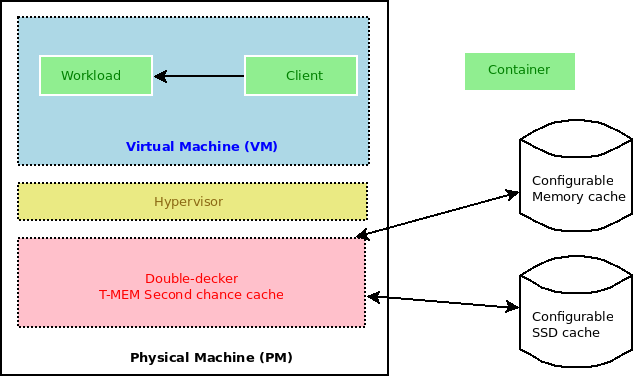
\includegraphics[width=0.9\textwidth]{images/correctness/exp_setup.png}
	  \caption{Experimental testbed for checking correctness}
	  \label{img_correctness_testbed}
	\end{figure}
  
    \subsection{Arithematic validation of stats}
    
    \subsection{Movement of objects between both levels of cache}
	
	\subsubsection{Memory to SSD cache}

	  \myparagraph{Question}
	    To verify the correctness in accounting of stats while accessing cache and moving objects from memory (L1) to SSD (L2) cache.
	    
	  \myparagraph{Procedure}
	    H
	
	\subsubsection{SSD to memory cache}
    
  
  
  
  \section{Evaluation of Double Decker}
  
    \subsection{Experimental setup}
	
	\paragraph{Experimental configurations}
	
	\paragraph{Metrics of interest}
	
	\paragraph{Workload}
	
	\paragraph{Testbed}
  
    \subsection{Provisioning for anonymous and file backed workloads}
    
    \subsection{Hybrid cache provisioning}
    
  % \chapter{Implementation details}
% 
%   \section{Modified memory Cgroup}
%   
%     \subsection{Per container configurable weights}
%     
%     \subsection{Deterministic reclamation}
%     
%     \subsection{Flexible reclamation size}
%     
%   
%   \section{Double decker}
%   
%     \subsection{Existing memory management framework}
%     
%     \subsection{Updations to exisiting framework}
%     
%       \subsubsection{Multilevel configurable caches}
%       
%       \subsubsection{Asyncronous kernel threads for transfer of objects}
%       
%       \subsubsection{Multilevel stats}
%   
  % 
% \chapter{Evaluation}
% 
%   \section{Updated memory Cgroup controller}
%   
%     \subsection{exp1}
%     \subsection{exp2}
%   
%   \section{Double decker}
%   
%     \subsection{exp1}
%     \subsection{exp2}
% 
%   
  
\chapter{Conclusions}
  
    We have made an initial attempt to understand memory management in Linux containers. We started off with purposing hypotheses based on 
theoretical evidences. We performed empirical analysis to verify the correctness of our purposed hypotheses. We also performed a few more 
empirical analysis to establish parts of memory management for which hypotheses couldn't be drawn. We then tried to extrapolate its 
implications in the real world applications running inside a derivative cloud environment. These implications strongly suggested that 
existing memory management techniques may impact higher provisioned containers negatively, when the system is under memory pressure. We 
conclude by purposing the requirements of a new desired policy that provides this notion of a differentiated reclamation to enforce 
deterministic allocation when the system is under memory pressure.  
  
 
  \chapter{Future Extensions}
  
    The following are the list of works that are to be taken up in the near future,
    
      \begin{enumerate}
	\item Design and implement a new memory management policy for containers.
	\item Analyze memory hierarchy in cgroups, and see how this affects containers.
	\item Explore other resource controller in the container framework, identify issues and provide appropriate fixes.
	\item The end goal is to provide an adaptive resource provisioning framework for containers. 
      \end{enumerate}

  

  
  \bibliographystyle{ieeetr}
  \bibliography{mylit}  
  
  %\appendix
  %\include{appendix/demos}
  %\include{appendix/benchmarks}

\end{document}

%%% Local Variables: 
%%% mode: latex
%%% TeX-master: t
%%% End: 
